\chapter{Результаты}
 
 Для ознакомления с программами мною были составлены входные файлы для всех трёх вышеупомянутых пакетов, рассчитывающие зонную структуру однородного бесконечного листа графена методами DFT. Использованные входные файлы для программ представлены в приложениях А, Б и В. Также, для обработки данных и визуализации зонной структуры мной был написан скрипт, представленный в приложении Г.

 Полученные результаты представлены на рисунке~\ref{res}.
 Из представленных графиков видно, что все три программы дают качественно правильные результаты. На всех трёх зонных структурах для двух верхних зон вблизи точки K наблюдается участок с линейной дисперсией -- конус Дирака. ABINIT и QUANTUM ESPRESSO дают почти идентичные результаты. Для нижних зон результаты совпадают, а для верхних расхождение составляет не более 0,3 эВ. Результаты CRYSTAL так же совпадают с другими на нижних зонах, но на верхних разница с двумя другими пакетами составляет более 1 эВ.

 В \cite{graphene} представлена иллюстрация зонной структуры графена изображённая на рисунке~\ref{lit}. Результаты, полученные с помощью ABINIT и QUANTUM ESPRESSO, хорошо соотносятся, с результатами, представленными на этом графике. CRYSTAL даёт завышенную энергию \( \pi \)-зон.

 \begin{figure}[h!]
    \center
    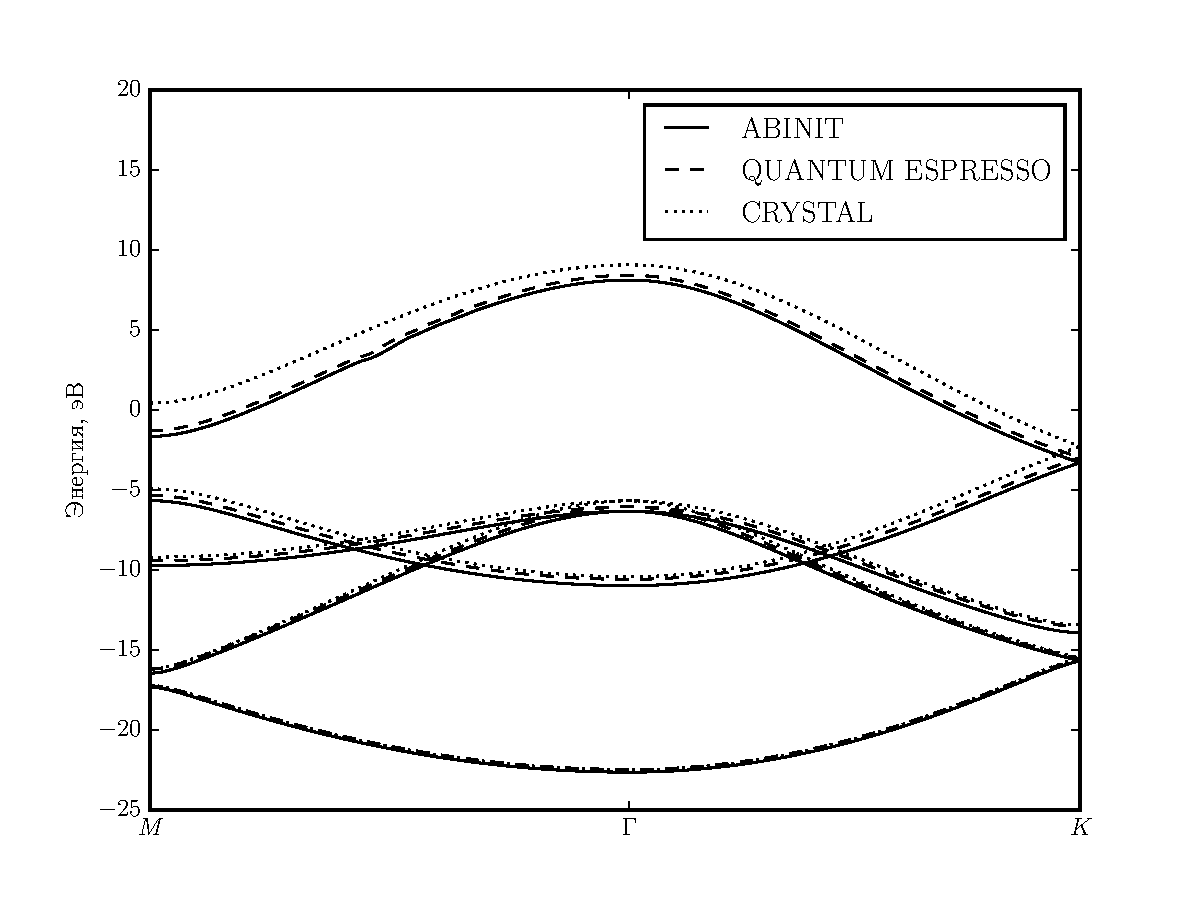
\includegraphics[width=.9\textwidth]{res}
    \caption{Зонная структура графена по результатам расчётов}
    \label{res}
\end{figure}
\vspace*{4cm}
\begin{figure}[h!]
    \center
    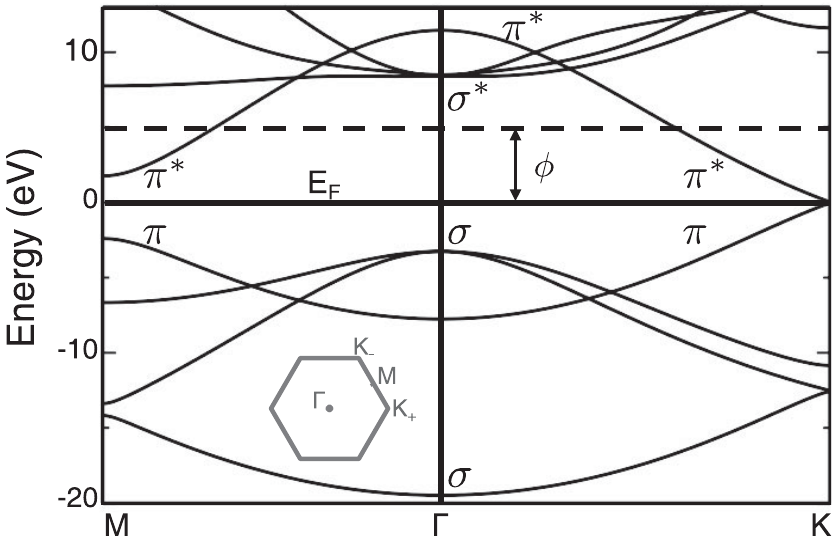
\includegraphics[width=.8\textwidth]{lit}
    \caption{Зонная структура графена, представленная в \cite{graphene}}
    \label{lit}
\end{figure}
\clearpage